% !TEX root = ../zavrsni_rad.tex

\chapter{Implementacija sustava}
\label{pog:implementacija}

\section{Arhitektura sustava}

Sustav je implementiran u Pythonu i organiziran u module koji odgovaraju logičkim slojevima arhitekture. Svaki modul ima jasno definiran ulaz i izlaz bez globalnog stanja. Sve konfiguracijske vrijednosti --- dimenzije okoline, parametri robota, horizonti i težine MPC-a --- čitaju se iz jedne datoteke \texttt{config/params.yaml}, čime je odvojena konfiguracija od logike.

Izvršavanje počinje u \texttt{src/scenarios.py}, koji za odabrani scenarij vraća rječnik s početnim stanjem robota, koordinatama cilja i popisom prepreka. Prepreke su definirane u \texttt{src/obstacles.py} kao instance klasa \texttt{Circle} i \texttt{Rectangle}. Pravokutne prepreke se interno aproksimiraju mrežom malih kružnica kako bi bile kompatibilne s acados-ovim sustavom nelinearnih ograničenja koji očekuje analitičke izraze u obliku $h(\mathbf{x}) \geq 0$.

Na temelju popisa prepreka i pozicija starta i cilja, \texttt{src/astar.py} gradi diskretiziranu mrežu okoline rezolucije $0{,}2$ m i markira sve čvorove koji su unutar infliranog radijusa prepreke kao zauzete. Algoritmom A* s euklidskom heuristikom i mogućnošću kretanja u osam smjerova pronalazi se kolizijsko-slobodna putanja u obliku niza čvorova mreže. Ako put ne postoji, algoritam baca iznimku i solver se ne pokreće.

Putanja dobivena A* algoritmom potom ulazi u \texttt{src/path\_smoother.py}. Funkcija \texttt{smooth} uklanja duplikate točaka i aproksimira ih kubičnim B-splineom s parametrom glađenja $s{=}0{,}5$, uzorkovanim na $200$ ravnomjerno raspoređenih točaka. Funkcija \texttt{velocity\_profile} zatim za svaku točku izglađene putanje procjenjuje zakrivljenost iz promjene smjera susjednih segmenata i postavlja referentnu brzinu obrnuto proporcionalnu zakrivljenosti --- uski zavoji za potrebe vizualizacije dobivaju nižu prikazanu referentnu brzinu; NMPC autonomno bira stvarnu brzinu unutar $v_{min} \leq v \leq v_{max}$.

Paralelno s planiranjem putanje, \texttt{src/model.py} definira simbolički CasADi model monocikla koji se predaje modulu \texttt{src/mpc\_solver.py}. Solver pri inicijalizaciji kreira acados \cite{verschueren2022acados} \texttt{AcadosOcp} objekt: postavlja matrice troška $Q$ i $R$, intervalna ograničenja na stanja i upravljanje te, ako scenarij ima prepreke, dodaje nelinearna ograničenja za svaku prepreku kao meko ograničenje s kaznenim faktorom $10^4$. Iz tog opisa acados generira i kompajlira optimizirani C kod solvera koji se koristi u simulaciji.

Sama simulacija odvija se u \texttt{src/simulation.py} kao zatvorena petlja opisana u odjeljku~\ref{sec:simloop}. Nakon završetka simulacije, \texttt{src/metrics.py} iz zabilježenih stanja, upravljanja i vremena rješavanja izračunava RMSE, CTE, grešku smjera i CPU statistiku. Rezultati se vizualiziraju modulima \texttt{src/plot.py} i \texttt{src/animate.py}.

Tijek podataka kroz sustav prikazan je na slici~\ref{slk:architecture}.

\begin{figure}[H]
  \centering
  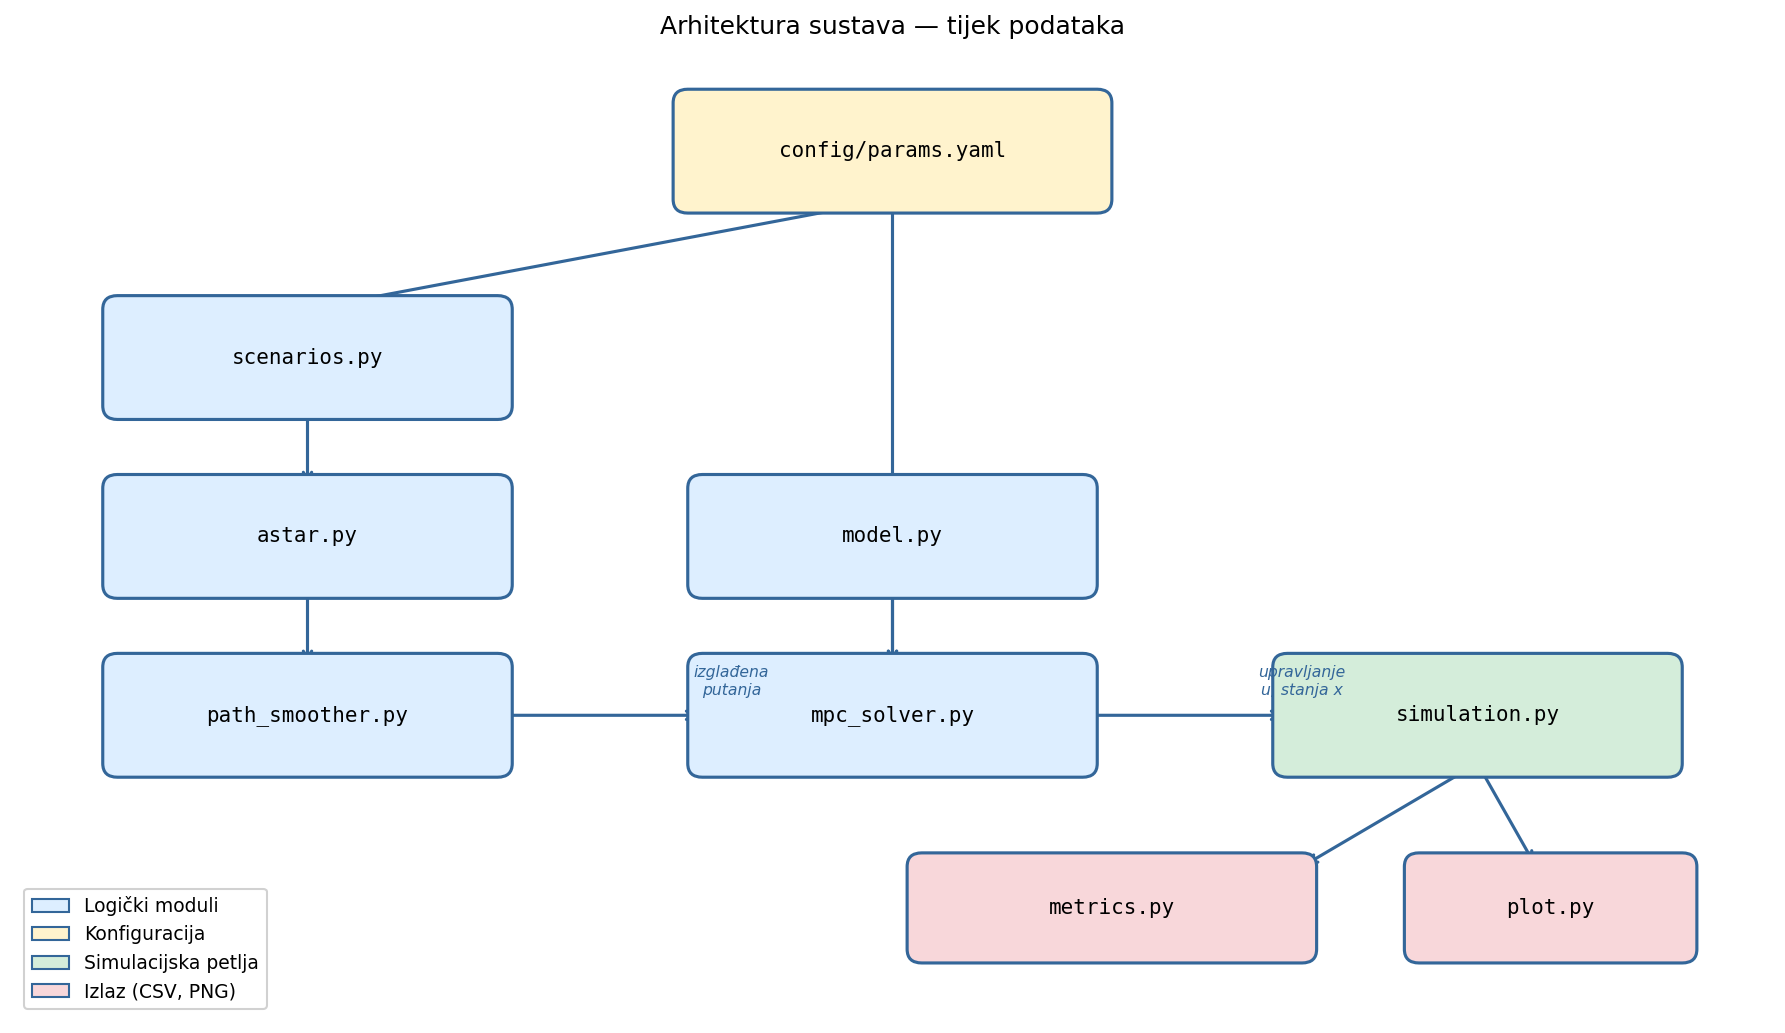
\includegraphics[width=0.95\linewidth]{figures/architecture.png}
  \caption{Arhitektura sustava. Konfiguracija (\texttt{params.yaml}) napaja sve module parametrima. Lijevi stupac prikazuje put planiranja putanje, sredina solver, a desno simulacijsku petlju i izlaz.}
  \label{slk:architecture}
\end{figure}

\section{Simulacijska petlja zatvorene petlje}
\label{sec:simloop}

Srž sustava je simulacijska petlja u \texttt{src/simulation.py}. Na svakom koraku:

\begin{enumerate}
  \item pronađe se najbliža sljedeća putna točka na putanji
  \item postavi se referenca $\mathbf{y}_{ref}$ za svih $N$ koraka horizonta
  \item fiksira se trenutno stanje kao početni uvjet OCP-a
  \item poziva se \texttt{solver.solve()} koji izvršava SQP\_RTI iteraciju
  \item uzima se prvi upravljački signal $\mathbf{u}_0^*$
  \item integrira se model RK4 metodom
  \item primjenjuje se eventualni poremećaj
\end{enumerate}

\begin{listing}[H]
\begin{minted}{python}
for step in range(max_steps):
    # napreduj do najbliže sljedeće putne točke
    while wp_idx < len(waypoints) - 1:
        if np.linalg.norm(x[:2] - waypoints[wp_idx+1]) \
                <= np.linalg.norm(x[:2] - waypoints[wp_idx]):
            wp_idx += 1
        else:
            break

    # postavi referencu za N koraka unaprijed
    for k in range(N):
        ref_idx = min(wp_idx + k, len(waypoints) - 1)
        xr, yr = waypoints[ref_idx]                    # koordinate ciljne putne točke
        dx = waypoints[min(ref_idx+1, len(waypoints)-1)][0] - xr
        dy = waypoints[min(ref_idx+1, len(waypoints)-1)][1] - yr
        theta_ref = np.arctan2(dy, dx)                 # smjer putanje u toj točki
        solver.set(k, "yref", np.array([xr, yr, theta_ref, 0.0, 0.0]))

    # fiksiraj trenutno stanje kao početni uvjet
    solver.set(0, "lbx", x)
    solver.set(0, "ubx", x)

    solver.solve()                    # jedna SQP_RTI iteracija
    u = solver.get(0, "u")           # uzmi prvi upravljački signal
    x = _rk4_step(x, u, dt)         # integriraj simulirani robot

    if np.linalg.norm(x[:2] - goal) < tol:
        break                         # cilj dosegnut
\end{minted}
\caption{Jezgra simulacijske petlje u \texttt{src/simulation.py}}
\end{listing}

\begin{figure}[H]
  \centering
  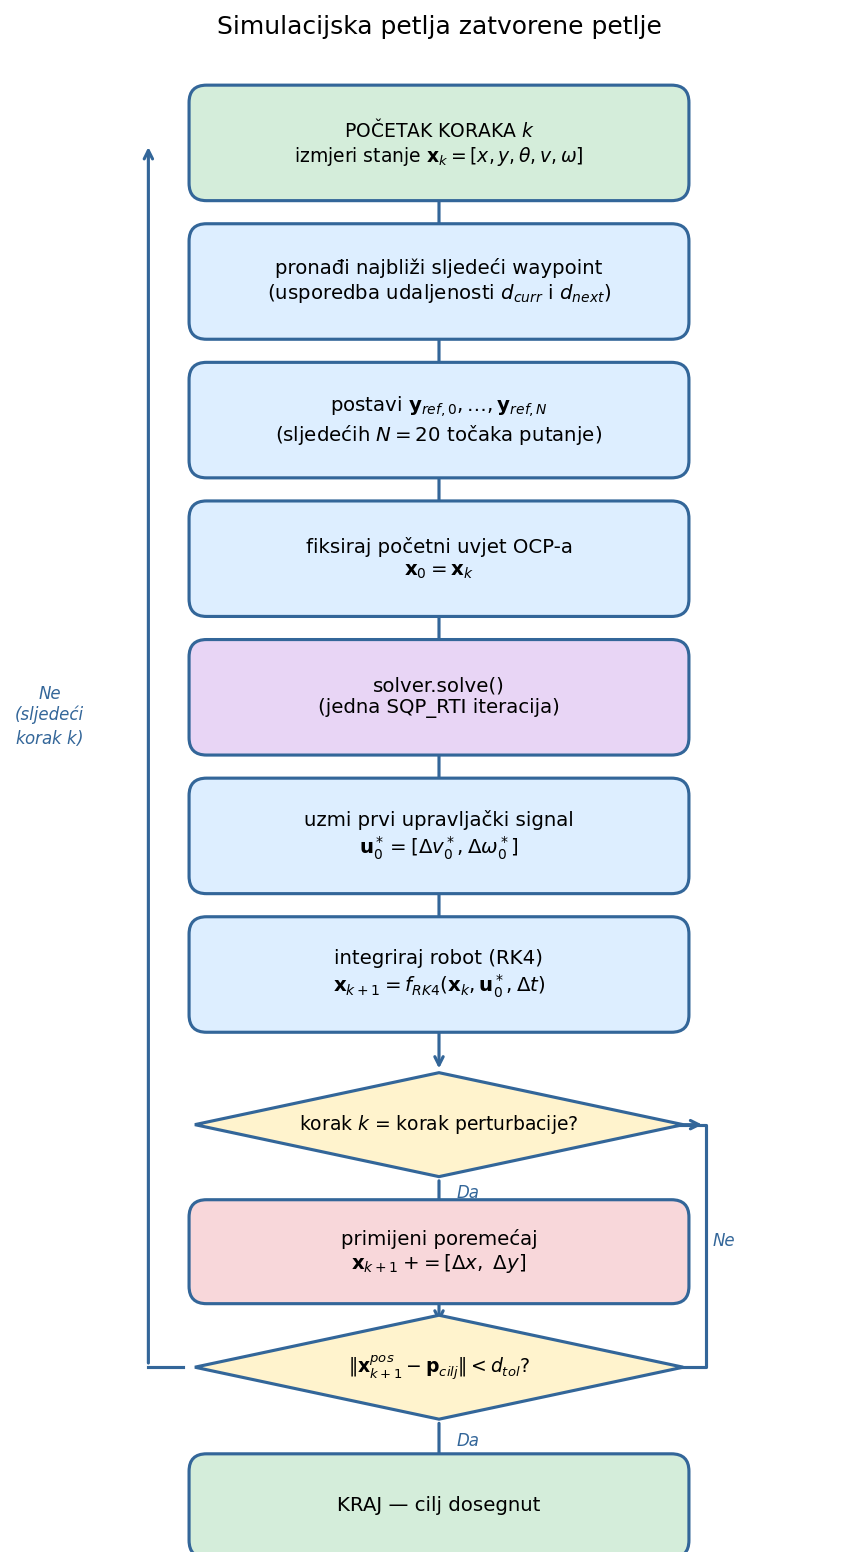
\includegraphics[width=0.52\linewidth]{figures/simulation_loop.png}
  \caption{Dijagram toka simulacijske petlje zatvorene petlje. Ljubičasti blok označava SQP\_RTI korak solvera, crveni blok primjenu poremećaja (prisutan samo u perturbacijskom scenariju).}
  \label{slk:simulation_loop}
\end{figure}

Napredak po putanji određuje se usporedbom udaljenosti. Na svakom koraku algoritam izračunava $d_{curr} = \|\mathbf{p} - \mathbf{w}_{idx}\|$ i $d_{next} = \|\mathbf{p} - \mathbf{w}_{idx+1}\|$ te pomiče indeks naprijed sve dok vrijedi $d_{next} \leq d_{curr}$. Uvjet se provjerava u petlji pa robot može preskočiti više putnih točaka odjednom pri većim brzinama. Slika~\ref{slk:waypoint_tracking} ilustrira mehanizam: dok je robot blizu $w_2$, vrijedi $d_{next} \gg d_{curr}$ i indeks stoji; čim robot prijeđe polovicu puta prema $w_3$, sljedeća putna točka postaje bliža i indeks se pomiče. Na taj način referentna točka uvijek odgovara stvarnoj poziciji robota u prostoru.

\begin{figure}[H]
  \centering
  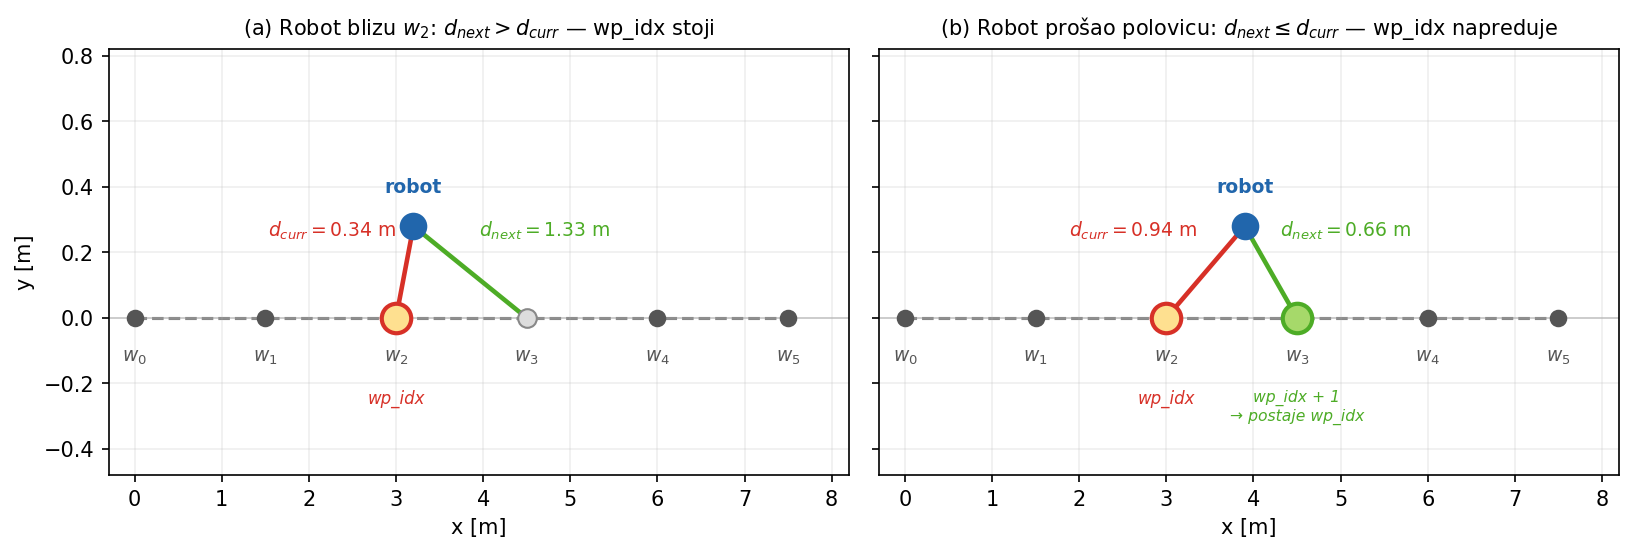
\includegraphics[width=0.95\linewidth]{figures/waypoint_tracking.png}
  \caption{Mehanizam napredovanja indeksa \texttt{wp\_idx}. Lijevo: robot je blizu $w_2$, vrijedi $d_{next} \gg d_{curr}$ i indeks stoji. Desno: robot je prešao polovicu segmenta prema $w_3$, vrijedi $d_{next} \leq d_{curr}$ i indeks napreduje.}
  \label{slk:waypoint_tracking}
\end{figure}

\section{Metrike kvalitete praćenja}

Modul \texttt{src/metrics.py} izračunava četiri mjere kvalitete iz rezultata simulacije.

\textbf{RMSE} (eng.\ \textit{Root Mean Square Error}) mjeri prosječno odstupanje od referentne putanje:

\begin{equation}
  \text{RMSE} = \sqrt{\frac{1}{K} \sum_{k=0}^{K-1} d_k^2}, \qquad d_k = \min_j \|\mathbf{p}_k - \mathbf{w}_j\|_2
\end{equation}

gdje je $d_k$ udaljenost od najbliže točke na putanji u koraku $k$. U implementaciji se za svaki vremenski korak izračunava udaljenost do svake točke izglađene putanje i uzima se minimum:

\begin{listing}[H]
\begin{minted}{python}
dists = np.linalg.norm(path - state[:2], axis=1)
idx   = np.argmin(dists)
d_k   = dists[idx]
\end{minted}
\caption{Izračun udaljenosti $d_k$ za RMSE u \texttt{src/metrics.py}}
\end{listing}

\textbf{CTE} (eng.\ \textit{Cross-Track Error}) mjeri okomitu udaljenost od segmenta putanje --- za razliku od RMSE-a uzima u obzir smjer putanje:

\begin{equation}
  \text{CTE}_k = \left| (\mathbf{p}_k - \mathbf{w}_{j^*}) \times \hat{\mathbf{t}}_{j^*} \right|
\end{equation}

gdje je $\hat{\mathbf{t}}_{j^*}$ smjer putanje u najbližoj točki $w_{j^*}$. Implementacija koristi skalarni oblik dvodimenzionalnog vektorskog produkta:

\begin{listing}[H]
\begin{minted}{python}
seg      = path[idx + 1] - path[idx]
seg_norm = seg / np.linalg.norm(seg)
diff     = state[:2] - path[idx]
cte      = abs(diff[0] * seg_norm[1] - diff[1] * seg_norm[0])
\end{minted}
\caption{Izračun CTE u \texttt{src/metrics.py}}
\end{listing}

\textbf{Greška smjera} (eng.\ \textit{heading error}) je apsolutna kutna razlika između orijentacije robota i smjera putanje, izračunata korištenjem atan2 za ispravno rukovanje kutnim prelaskom:

\begin{equation}
  e_{\theta,k} = \left| \text{atan2}(\sin(\theta_k - \theta_{ref,k}),\ \cos(\theta_k - \theta_{ref,k})) \right|
\end{equation}

Direktno oduzimanje kutova $\theta_k - \theta_{ref,k}$ nije ispravno jer rezultat može izaći iz intervala $(-\pi, \pi]$; formulacija s funkcijom \texttt{atan2} osigurava da greška uvijek ostaje unutar tog intervala.

\begin{listing}[H]
\begin{minted}{python}
theta_ref = np.arctan2(seg[1], seg[0])
he = abs(np.arctan2(np.sin(state[2] - theta_ref),
                     np.cos(state[2] - theta_ref)))
\end{minted}
\caption{Izračun greške smjera u \texttt{src/metrics.py}}
\end{listing}

Geometrijska interpretacija sve tri mjere prikazana je na slici~\ref{slk:metrics_concept}.

\begin{figure}[H]
  \centering
  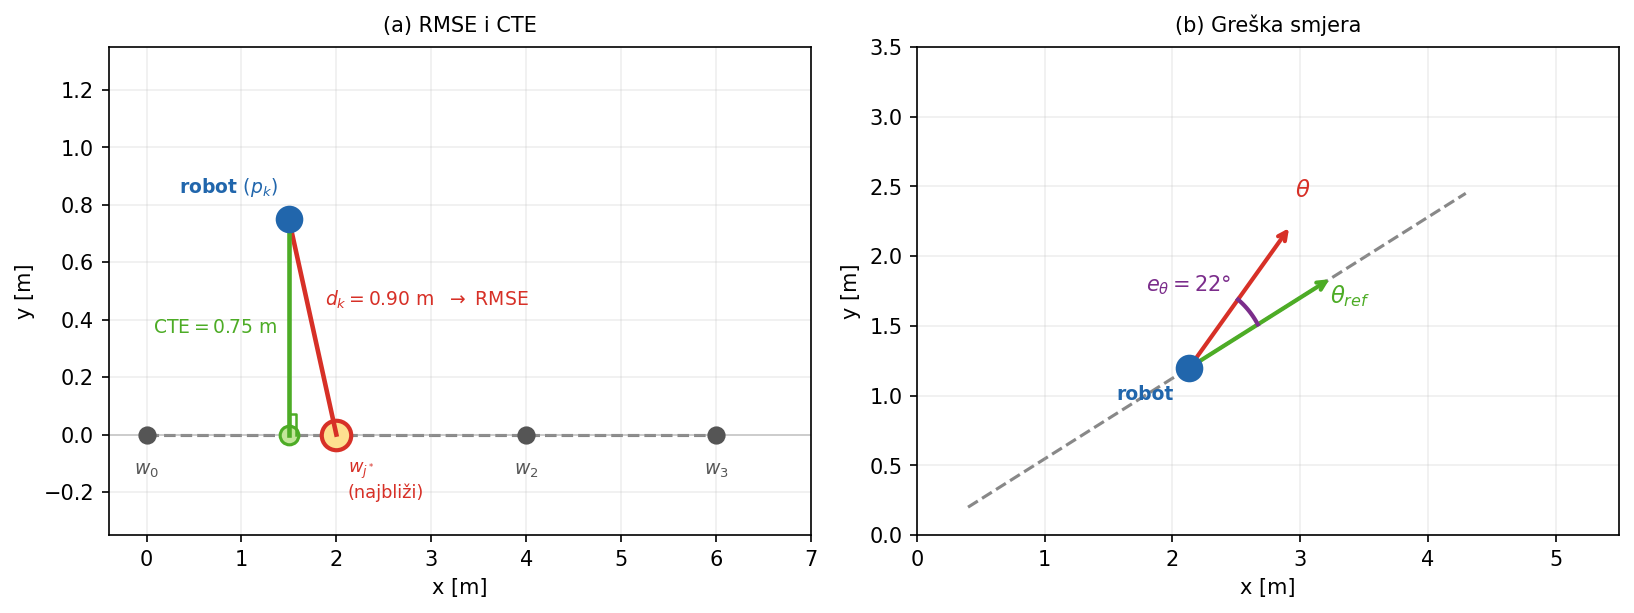
\includegraphics[width=0.95\linewidth]{figures/metrics_concept.png}
  \caption{Geometrijska interpretacija mjera kvalitete. Lijevo: RMSE mjeri udaljenost do najbliže putne točke $w_{j^*}$ (crvena linija $d_k$), dok CTE mjeri okomitu udaljenost do segmenta putanje (zelena linija). Desno: greška smjera $e_\theta$ je kutna razlika između orijentacije robota $\theta$ i referentnog smjera putanje $\theta_{ref}$.}
  \label{slk:metrics_concept}
\end{figure}

\textbf{CPU vrijeme} mjeri se funkcijom \texttt{time.perf\_counter()} neposredno oko svakog poziva \texttt{solver.solve()}, a bilježe se prosječno i maksimalno vrijeme po simulaciji:

\begin{listing}[H]
\begin{minted}{python}
t0 = time.perf_counter()
solver.solve()
solve_times.append(time.perf_counter() - t0)
\end{minted}
\caption{Mjerenje CPU vremena jedne SQP\_RTI iteracije u \texttt{src/simulation.py}}
\end{listing}

\section{Testni scenariji}

Sustav je testiran na osam scenarija različite složenosti: sedam u kojima robot uspješno dostiže cilj te jedan (\texttt{blocked}) koji testira prepoznavanje neizvedivog puta. U preostalim poglavljima pojam ``sedam scenarija'' odnosi se na ovih sedam navigacijskih scenarija, isključujući \texttt{blocked}. Tablica~\ref{tab:scenariji} prikazuje ključne karakteristike svih osam scenarija.

\begin{table}[H]
\centering
\caption{Pregled testnih scenarija}
\label{tab:scenariji}
\begin{tabular}{llll}
\toprule
Scenarij & Start & Cilj & Prepreke \\
\midrule
baseline     & $(0{,}5;\; 0{,}5)$ & $(9{,}5;\; 9{,}5)$ & — \\
one\_obstacle & $(0{,}5;\; 0{,}5)$ & $(9{,}5;\; 9{,}5)$ & 1 krug $r=1{,}0$ m \\
narrow       & $(0{,}5;\; 5{,}0)$ & $(9{,}5;\; 5{,}0)$ & 2 kruga $r=1{,}2$ m \\
l\_corridor  & $(0{,}5;\; 1{,}0)$ & $(9{,}0;\; 9{,}0)$ & 1 pravokutnik \\
u\_shape     & $(5{,}0;\; 0{,}5)$ & $(5{,}0;\; 9{,}5)$ & 3 pravokutnika \\
perturbation & $(0{,}5;\; 5{,}0)$ & $(9{,}5;\; 5{,}0)$ & — ($\Delta y = +1{,}0$ m u $t=3$ s) \\
cluttered    & $(0{,}5;\; 0{,}5)$ & $(9{,}5;\; 9{,}5)$ & 7 krugova \\
blocked      & $(0{,}5;\; 5{,}0)$ & $(9{,}5;\; 5{,}0)$ & 5 krugova (zid) \\
\bottomrule
\end{tabular}
\end{table}

Scenarij \texttt{blocked} je poseban --- A* ne može pronaći put pa se NMPC solver uopće ne pokreće. Sustav to prepoznaje i prikazuje kartu s porukom o neizvedivosti, što je opisano u poglavlju~\ref{pog:rezultati}.

Svaki scenarij definiran je kao Python rječnik koji vraća funkcija u \texttt{src/scenarios.py}. Primjer scenarija s uskim prolazom između dviju kružnih prepreka:

\begin{listing}[H]
\begin{minted}{python}
def _narrow():
    return {
        "name": "narrow",
        "start": np.array([0.5, 5.0, 0.0]),
        "goal":  np.array([9.5, 5.0]),
        "obstacles": [
            Circle(5.0, 3.5, 1.2),
            Circle(5.0, 6.5, 1.2),
        ],
        "perturbation": None,
    }
\end{minted}
\caption{Definicija scenarija uskog prolaza u \texttt{src/scenarios.py}. Prepreke su instance klase \texttt{Circle(cx, cy, r)}; svi scenariji bez poremećaja imaju \texttt{perturbation: None}.}
\end{listing}
